% Drawing 156-6/04-7 -- folder 156-6, batch 04, archive page 79 (PDF page 80).
% Transcription: schéma d'implications : de « At $9_{\Sigma}$ $+$ At 10 » partent deux doubles flèches, vers At $9_{\Sigma}$ et vers At 12 ; de At $9_{\Sigma}$ une double flèche vers At 9 (critère de disj.\ par les lieux) ; de At 12 deux doubles flèches, vers At 10 et vers At 11' ; de At 11 une double flèche vers At 11'. Les légendes sont transcrites ci-dessous
% Kind: diagram of implications from At 9_Sigma + At 10. Method 2 (schematic redraw from the facsimile). Status: ok.
% Notes: From "At 9_Sigma + At 10" two double arrows (drawn single), to At 9_Sigma and to At 12; At 9_Sigma => At 9 (critere de disj. par les lieux); At 12 => At 10 and => At 11'; At 11 => At 11'. The captions on the right (recollement des raffinements ...) are given in short as on the page.
% Coordinates: 1 unit = 1 mm = 1/100 of the crop width (bbox in page fractions: [0.25, 0.6, 0.95, 0.75]).
% Redrawn by Claude (claude-opus-5-5), issue #73, 2026-11-07; not checked by a human; not compiled (no TeX in the session).
% Rights: reproduces part of the work -- behind RENDER_TRANSCRIPTS, never published by itself.
\documentclass[tikz,border=3pt]{standalone}
\usepackage{amsmath,amssymb}
\usetikzlibrary{patterns,arrows.meta}
\tikzset{pencil/.style={black!45}, struck/.style={black!35}, mark/.style={circle,draw,inner sep=1.3pt}, pt/.style={circle,fill,inner sep=0.9pt}, opt/.style={circle,draw,fill=white,inner sep=1.1pt}}
\begin{document}
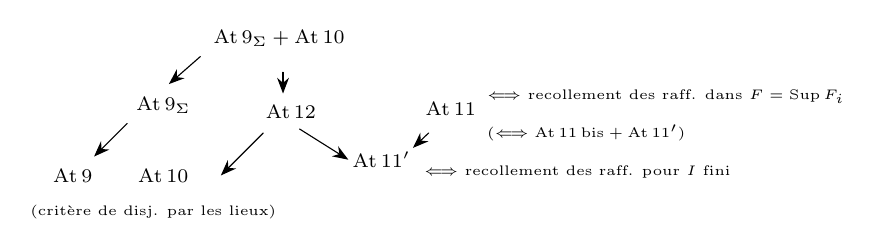
\begin{tikzpicture}[x=1mm,y=1mm,line cap=round,line join=round,font=\scriptsize]
\node[inner sep=1pt] at (37,-6.5) {\scriptsize $\mathrm{At}\,9_\Sigma+\mathrm{At}\,10$};
\node[inner sep=1pt] at (22.3,-15) {\scriptsize $\mathrm{At}\,9_\Sigma$};
\node[inner sep=1pt] at (38.5,-15.8) {\scriptsize $\mathrm{At}\,12$};
\node[inner sep=1pt] at (58.8,-15.4) {\scriptsize $\mathrm{At}\,11$};
\node[inner sep=1pt] at (10.8,-23.9) {\scriptsize $\mathrm{At}\,9$};
\node[inner sep=1pt] at (22.3,-23.9) {\scriptsize $\mathrm{At}\,10$};
\node[inner sep=1pt] at (50,-21.9) {\scriptsize $\mathrm{At}\,11'$};
\draw[-{Stealth[length=2mm]}] (27,-8.8) -- (23,-12.3);
\draw[-{Stealth[length=2mm]}] (37.5,-10.8) -- (37.5,-13.5);
\draw[-{Stealth[length=2mm]}] (17.7,-17.3) -- (13.5,-21.5);
\draw[-{Stealth[length=2mm]}] (35,-18.5) -- (29.6,-23.9);
\draw[-{Stealth[length=2mm]}] (39.6,-18) -- (45.8,-21.9);
\draw[-{Stealth[length=2mm]}] (56,-18.5) -- (54,-20.4);
\node[inner sep=1pt,anchor=west] at (5,-28.5) {\tiny (critère de disj. par les lieux)};
\node[inner sep=1pt,anchor=west] at (63,-13.9) {\tiny $\Longleftrightarrow$ recollement des raff. dans $F=\mathrm{Sup}\,F_i$};
\node[inner sep=1pt,anchor=west] at (63,-18.5) {\tiny $(\Longleftrightarrow \mathrm{At}\,11\,\mathrm{bis}+\mathrm{At}\,11')$};
\node[inner sep=1pt,anchor=west] at (55,-23.5) {\tiny $\Longleftrightarrow$ recollement des raff. pour $I$ fini};
\end{tikzpicture}
\end{document}
